\documentclass[11pt,openright,twoside,french]{book}
\usepackage{marvosym}
\input philippe2013
\input philippe2013_activites
\pagestyle{empty}


\begin{document}

\TitreActivite{xii.1}{Fonctions polynômes \\ de degré 2}\medskip

À l'aide de la calculatrice, on a représenté plusieurs fonctions :
\begin{center}
    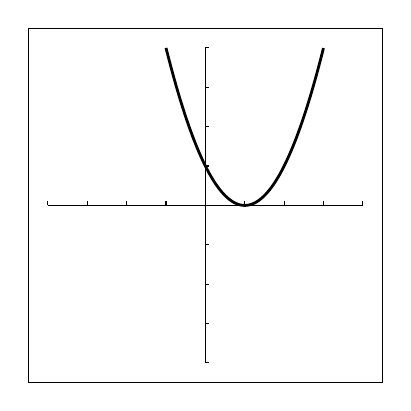
\begin{tikzpicture}[scale=0.5]
        \def\xmin{-4}\def\xmax{4}
        \def\ymin{-4}\def\ymax{4}
        \draw (\xmin,0) -- (\xmax,0); \foreach \x in {\xmin,...,\xmax} \draw (\x,0) -- (\x,0.1);
        \draw (0,\ymin) -- (0,\ymax); \foreach \x in {\ymin,...,\ymax} \draw (0,\x) -- (0.1,\x);
        \draw[smooth,samples=200,domain=-1:3, line width = 1pt] plot(\x,{(\x-1)^2});
        \draw (\xmin-0.5,\ymin-0.5) rectangle (\xmax + .5,\ymax + .5);
    \end{tikzpicture}\qquad
    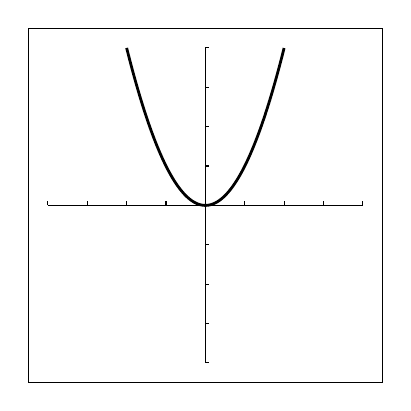
\begin{tikzpicture}[scale=0.5]
        \def\xmin{-4}\def\xmax{4}
        \def\ymin{-4}\def\ymax{4}
        \draw (\xmin,0) -- (\xmax,0); \foreach \x in {\xmin,...,\xmax} \draw (\x,0) -- (\x,0.1);
        \draw (0,\ymin) -- (0,\ymax); \foreach \x in {\ymin,...,\ymax} \draw (0,\x) -- (0.1,\x);
        \draw[smooth,samples=200,domain=-2:2, line width = 1pt] plot(\x,{(\x)^2});
        \draw (\xmin-0.5,\ymin-0.5) rectangle (\xmax + .5,\ymax + .5);
    \end{tikzpicture}\qquad
    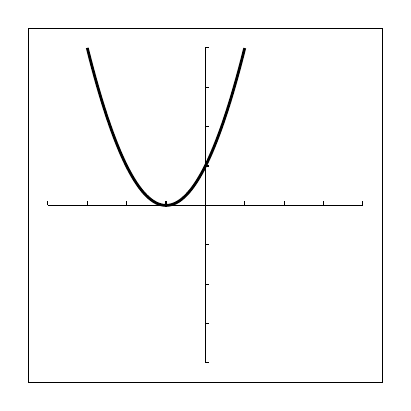
\begin{tikzpicture}[scale=0.5]
        \def\xmin{-4}\def\xmax{4}
        \def\ymin{-4}\def\ymax{4}
        \draw (\xmin,0) -- (\xmax,0); \foreach \x in {\xmin,...,\xmax} \draw (\x,0) -- (\x,0.1);
        \draw (0,\ymin) -- (0,\ymax); \foreach \x in {\ymin,...,\ymax} \draw (0,\x) -- (0.1,\x);
        \draw[smooth,samples=200,domain=-3:1, line width = 1pt] plot(\x,{(\x+1)^2});
        \draw (\xmin-0.5,\ymin-0.5) rectangle (\xmax + .5,\ymax + .5);
    \end{tikzpicture}\bigskip
    
    \begin{tikzpicture}[scale=0.5]
        \def\xmin{-4}\def\xmax{4}
        \def\ymin{-4}\def\ymax{4}
        \draw (\xmin,0) -- (\xmax,0); \foreach \x in {\xmin,...,\xmax} \draw (\x,0) -- (\x,0.1);
        \draw (0,\ymin) -- (0,\ymax); \foreach \x in {\ymin,...,\ymax} \draw (0,\x) -- (0.1,\x);
        \draw[smooth,samples=200,domain=-1.5:1.5, line width = 1pt] plot(\x,{(\x)^2+2});
        \draw (\xmin-0.5,\ymin-0.5) rectangle (\xmax + .5,\ymax + .5);
    \end{tikzpicture}\qquad
    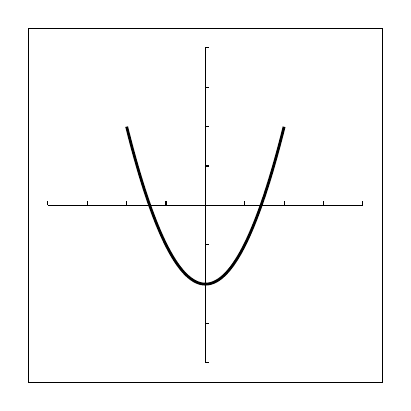
\begin{tikzpicture}[scale=0.5]
        \def\xmin{-4}\def\xmax{4}
        \def\ymin{-4}\def\ymax{4}
        \draw (\xmin,0) -- (\xmax,0); \foreach \x in {\xmin,...,\xmax} \draw (\x,0) -- (\x,0.1);
        \draw (0,\ymin) -- (0,\ymax); \foreach \x in {\ymin,...,\ymax} \draw (0,\x) -- (0.1,\x);
        \draw[smooth,samples=200,domain=-2:2, line width = 1pt] plot(\x,{(\x)^2-2});
        \draw (\xmin-0.5,\ymin-0.5) rectangle (\xmax + .5,\ymax + .5);
    \end{tikzpicture}\qquad
    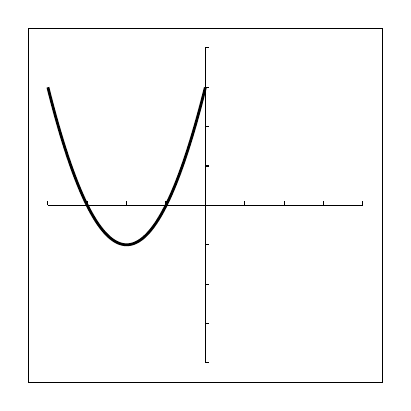
\begin{tikzpicture}[scale=0.5]
        \def\xmin{-4}\def\xmax{4}
        \def\ymin{-4}\def\ymax{4}
        \draw (\xmin,0) -- (\xmax,0); \foreach \x in {\xmin,...,\xmax} \draw (\x,0) -- (\x,0.1);
        \draw (0,\ymin) -- (0,\ymax); \foreach \x in {\ymin,...,\ymax} \draw (0,\x) -- (0.1,\x);
        \draw[smooth,samples=200,domain=-4:0, line width = 1pt] plot(\x,{(\x+2)^2-1});
        \draw (\xmin-0.5,\ymin-0.5) rectangle (\xmax + .5,\ymax + .5);
    \end{tikzpicture}
\end{center}

\begin{enumerate}
    \item Trouver des points communs entre toutes ces courbes ?
    \item Quelle courbe est la représentation de la fonction carré ?
    \item On considère les fonctions suivantes :
    \[f\colon x \mapsto (x +1)^2 \qetq g\colon x \mapsto (x - 1)^2\]
    \begin{enumerate}
        \item Retrouver les courbes représentant ces fonctions.
        \item Que remarque-t-on ?
        \item Déterminer le minimum de chacune de ses fonctions ? Pour quelle abscisse est-il atteint ?
    \end{enumerate}
    \item On considère les fonctions suivantes :
    \[u\colon x \mapsto x^2 + 2 \qetq v\colon x \mapsto x^2 - 2\]
    \begin{enumerate}
        \item Retrouver les courbes représentant ces fonctions.
        \item Que remarque-t-on ?
        \item Déterminer le minimum de chacune de ses fonctions ? Pour quelle abscisse est-il atteint ?
    \end{enumerate}
    \item
    \begin{enumerate}
        \item \'Ecrire les fonctions $f$, $g$, $u$ et $v$ sous la forme $(x - \alpha)^2 + \beta$ en donnant à chaque fois la valeur des nombres $\alpha$ et $\beta$.
        \item Quel lien existe-t-il à chaque fois entre $\alpha$, $\beta$ et le minimum de la fonction ?
    \end{enumerate}
    \item Le dernier graphique est la représentation d'une fonction $h$ inconnue.\par
    À l'aide des questions précédentes, déterminer l'expression de la fonction $h$.
\end{enumerate}
\end{document} 